%!TEX TS-program = xelatex
\documentclass[]{friggeri-cv}
\usepackage{afterpage}
\usepackage{hyperref}
\usepackage{color}
\usepackage{xcolor}
\hypersetup{
    pdftitle={},
    pdfauthor={},
    pdfsubject={},
    pdfkeywords={},
    colorlinks=false,       % no lik border color
   allbordercolors=white    % white border color for all
}
\addbibresource{bibliography.bib}
\RequirePackage{xcolor}
\definecolor{pblue}{HTML}{0395DE}

\begin{document}
\header{Paulo}{Rodrigues}
      {Programador}
      
% Fake text to add separator      
\fcolorbox{white}{gray}{\parbox{\dimexpr\textwidth-2\fboxsep-2\fboxrule}{%
.....
}}

% In the aside, each new line forces a line break
\begin{aside}
  \section{Endereço}
    Rua buique
    245, Piedade, Jaboatão dos Guararapes
    ~
  \section{Tel}
    +55 81 995261010
   ~
  \section{Links diretos}
    \href{mailto:pvrg.ava@gmail.com}{\textbf{Email@}\\gmail.com}
    \href{https://wa.me/5581995261010}{\textbf{Paulo Rodrigues@}\\whatsapp}
    ~
  \section{Web \& Git}
    \href{https://www.linkedin.com/in/paulorodrigues99/}{linkedin}
    \href{https://github.com/paulorodrigues99}{github}
    ~
  \section{Linguagens de Programação}
    \textbf{JavaScript}
\includegraphics[scale=0.40]{img/3stars.png}
    \textbf{Csharp}
\includegraphics[scale=0.40]{img/4stars.png}
    \textbf{AutoIt}
\includegraphics[scale=0.40]{img/3stars.png}
    ~
  \section{Habilidades}
    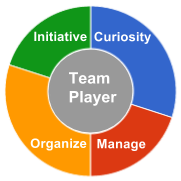
\includegraphics[scale=0.62]{img/personal.png}
    ~
  \section{Idiomas}
    \textbf{Espanhol}
\includegraphics[scale=0.40]{img/3stars.png}
    \textbf{Inglês}
\includegraphics[scale=0.40]{img/4stars.png}
\end{aside}

\section{Experiencia}
\begin{entrylist}
  \entry
    {06/17 - 08/19}
    {Associate Software Engineer}
    {\href{https://www.avanade.com/pt-br}{Avanade, Recife, Pernambuco}}
    {Profissional com atuação voltada ao Desenvolvimento de Software, formado em Gestão de Tecnologia da Informação. Participei de projetos de desenvolvimento de software e RPA, sugeri arquiteturas para problemas utilizando RPA.
Desenvolvi soluções utilizando as seguintes tecnologias: Csharp, Javascript, NodeJs, implementando Entity Framework, ReactJs e Express.

Desenvolvimento voltado a banco de dados com: SQL Server e MongoDb

Conhecimento da cultura de desenvolvimento ágil, utilizando as principais metodologias ágeis para gestão e planejamento dos projetos, através de ferramentas como TFS, Trello, SVN e Git.}
\end{entrylist}

\section{Educação}
\begin{entrylist}
  \entry
    {2017 - 2019}
    {Tecnologo em gestão de t.i}
    {\href{https://unifg.edu.br/}{Faculdade dos Guararapes, Jaboatão dos guararapes}}
    {}
\end{entrylist}

\section{Certificações}
\begin{entrylist}
  \entry
    {08/2019}
    {Bot Developer}
    {\href{https://certificates.automationanywhere.com/d4efdc40-8468-4d69-8508-b6d0be2068c4}{Automation Anywhere}}
    {\emph{Essa faixa ensina os desenvolvedores a entender os requisitos de negócios, identificar oportunidades de RPA, gerenciar o escopo do projeto e desenvolver e implantar automações usando os comandos internos do Automation Anywhere Enterprise para fornecer uma rápida resposta aos requisitos de negócios.}}
    \entry
    {08/2019}
    {Business Analyst}
    {\href{https://certificates.automationanywhere.com/60bdab56-89aa-4043-aee6-20ad65fd493a}{Automation Anywhere}}
    {\emph{Essa certificação ensina aos analistas de negócios como identificar os processos corretos para automação, calcular os benefícios do FTE e criar estimativas de esforço, documentar e justificar casos de uso, entender riscos e dependências e orientar os clientes no design do processo de automação.}}
    \entry
    {12/2018}
    {DEVOPS ESSENTIALS PROFESSIONAL CERTIFICATE (DEPC)}
    {CertiProf®}
    
    \entry
    {12/2018}
    {SCRUM FUNDATION PROFESSIONAL CERTIFICATE(SFPC)}
    {CertiProf®}
    
\end{entrylist}

\section{Iniciativas}
\href{https://www.portosocial.com.br/incubados/}{ONG Cidade que queremos:}\\
\emph{Inscrevemos o projeto CIDADE QUE QUEREMOS no Porto Social e fomos uma das 50 primeiras organizações sociais a participar da incubadora de negócios sociais. Realizamos uma ação no MÊS DAS CRIANÇAS e 1 evento no bairro de Candeias.Nosso projeto consiste em uma rede de associados com o objetivo de arrecadar recursos pra diversos projetos de financiamento coletivo.}
\section{Projetos}
\begin{entrylist}
    \entry
    {06-2017}
    {White marthins - POC}
    {Rafael Barros}
    {\emph{Projeto de automação em Blue Prism para auxilio na emissão de relatórios.}}
    \entry{09-2017}{LDC}{Francisco Pedroso}{\emph{Projeto de automação para atribuição de funcões para usuarios SAP.}}
    \entry{01-2018}{Coca-Cola}{Rafael Barros}{Projeto de automação de processos desenvolvido em Blue Prism para consulta de Multas nos sites do Detran dos 26 estados e Cadastro de Clientes no ERP SAP.}
    \entry{06-2018}{App Seu CA Powerapp Interno}{Rafael Barros}{Aplicativo para conectar profissionais de niveis de carreira diferente com o objetivo de gerar maior valor no programa da avanade de Conselheiros de Carreira }
    \entry{06-2018}{App Ubertime Powerapp Interno}{Rafael Barros}{Aplicativo para conectar profissionais com habilidades para atender demandas de horas extras, conectando gerentes de projetos com horas a ofertar e profissionais com interesse de atuar sobre as tecnologias ofertadas.}
    \entry{08-2018}{Ambev Fahz}{Alexandre}{Desenvolvimento, arquitetura e suporte com atendimento de chamados e apoio a operação de projeto em Blue Prism, solução para auditoria de planos de saúde e liberação do plano para o colaborador.}
    \entry{01-2019}{Tubos e conexões Tigre}{Rafael Barros}{Desenvolvimento em Automation Anywhere e CSharp para uma solução fim-a-fim de auditoria fiscal. Suporte a operação com os incidentes relacionados ao sistema e a automação via Jira.}
    \entry{07-2019}{Vale}{Bianca}{Desenvolvimento de Reporting Service e suporte a aplicações em Csharp.}

\end{entrylist}
\end{document}
